\newpage
\rhead{\textbf{\textcolor{blue}{Т}\textcolor{gray}{ерминология: Информация и данные}}}
\makebox[0em][l]{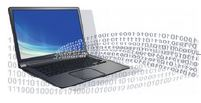
\includegraphics[scale=0.5]{1} }

\vspace*{5mm}
 Международный стандарт ISO/IEC 2382:2015\\
«Information technology – Vocabulary» (вольный пересказ):\\
\quad \quad \quad \textbf{\textcolor{Green}{Информация}} – знания относительно фактов, событий, \\ 
\quad \quad \quad вещей, идей и  понятий.\\
\quad \quad \quad \textbf{\textcolor{Green}{Данные}} – форма представления информации в виде, \\ 
\quad \quad \quad пригодном для передачи или обработки. \\
\vspace*{3mm}
$\bullet$ \quad Что есть предмет информатики: информация или данные? \\
$\bullet$ \quad Как измерить информацию? Как измерить данные?\\	
\qquad Пример: «Байкал — самое глубокое озеро Земли».
